%%%%%%%%%%%%%%%%%%%%%%%%%%%%%%%%%%%%%%%%%%%%%%%
%%% Template for lab reports used at STIMA
%%%%%%%%%%%%%%%%%%%%%%%%%%%%%%%%%%%%%%%%%%%%%%%

%%%%%%%%%%%%%%%%%%%%%%%%%%%%%% Sets the document class for the document
% Openany is added to remove the book style of starting every new chapter on an odd page (not needed for reports)
\documentclass[10pt,swedish, openany]{book}

%%%%%%%%%%%%%%%%%%%%%%%%%%%%%% Loading packages that alter the style
\usepackage[]{graphicx}
\usepackage[]{color}
\usepackage{alltt}
\usepackage[T1]{fontenc}
\usepackage[utf8]{inputenc}
\setcounter{secnumdepth}{3}
\setcounter{tocdepth}{3}
\setlength{\parskip}{\smallskipamount}
\setlength{\parindent}{0pt}
\usepackage{amsmath}
\usepackage{amssymb,latexsym}
\usepackage{mathtools}
\usepackage{subcaption}


% Set page margins
\usepackage[top=100pt,bottom=100pt,left=68pt,right=66pt]{geometry}

% Package used for placeholder text
\usepackage{lipsum}

% Prevents LaTeX from filling out a page to the bottom
\raggedbottom

% Adding both languages, Swedish and English, so they can be used intermittently in for example abstracts.
\usepackage[swedish, english]{babel}

% All page numbers positioned at the bottom of the page
\usepackage{fancyhdr}
\fancyhf{} % clear all header and footers
\fancyfoot[C]{\thepage}
\renewcommand{\headrulewidth}{0pt} % remove the header rule
\pagestyle{fancy}

% Changes the style of chapter headings
\usepackage{titlesec}
\titleformat{\chapter}
   {\normalfont\LARGE\bfseries}{\thechapter.}{1em}{}
% Change distance between chapter header and text
\titlespacing{\chapter}{0pt}{50pt}{2\baselineskip}

% Adds table captions above the table per default
\usepackage{float}
\floatstyle{plaintop}
\restylefloat{table}

% Adds space between caption and table
\usepackage[tableposition=top]{caption}

% Adds hyperlinks to references and ToC
\usepackage{hyperref}
\hypersetup{hidelinks,linkcolor = black} % Changes the link color to black and hides the hideous red border that usually is created

% If multiple images are to be added, a folder (path) with all the images can be added here 
\graphicspath{ {images/} }

% Separates the first part of the report/thesis in Roman numerals
\frontmatter

% add some useful definitions
\def\MeV{\ifmmode {\mathrm{\ Me\kern -0.1em V}}\else
                   \textrm{Ge\kern -0.1em V}\fi}%  

\def\GeV{\ifmmode {\mathrm{\ Ge\kern -0.1em V}}\else
                   \textrm{Ge\kern -0.1em V}\fi}%  

%%%%%%%%%%%%%%%%%%%%%%%%%%%%%% Starts the document
\begin{document}

%%% Selects the language to be used for the first couple of pages
\selectlanguage{english}

%%%%% Adds the title page
\begin{titlepage}
	\clearpage\thispagestyle{empty}
	\centering
	\vspace{2cm}

	% Titles
	{\large  \par}
	\vspace{8cm}
        {\Huge \textbf{Parity Violation in $\beta$ desintegrations}} \\
	\vspace{1cm}
	{\large \textbf{Laboratoire IV} \par}
	\vspace{2cm}
	{\large Luiza Ciucu \\ % \\ specifies a new line
	             Ana Ventura Barroso \par}
	\vspace{4cm}

    
\includegraphics[scale=0.75]{logo.jpg}
    
    \vspace{4cm}
    
	% Information about the University
	{\normalsize Universit\'e de Gen\`eve \\ 
		Facult\'e de Sciences \\
		Section de physique \\
		D\'epartement de Physique Nucl\'eaire et Corpusculaire \par}
		
	% Set the date
	{\normalsize 29-10-2019 \par}
	\vspace{2cm}
	
	\pagebreak

\end{titlepage}

% Adds a table of contents
\tableofcontents{}

\clearpage

\listoffigures

\clearpage


%%%%%%%%%%%%%%%%%%%%%%%%%%%%%%%%%%%%%%%%%%%%%%%%%%%%%%%%%%%%%%%%%%%%%%%%%%%%%%%%%%%%%%%%%%%%
%%%%%%%%%%%% The rows above should not be changed except for the title page information
%%%%%%%%%%%%%%%%%%%%%%%%%%%%%%%%%%%%%%%%%%%%%%%%%%%%%%%%%%%%%%%%%%%%%%%%%%%%%%%%%%%%%%%%%%%%
%%%%% Text body starts here!
\mainmatter

\chapter{Introduction}

``Nowadays, with broken symmetry almost universally accepted as a way of life, it is perhaps difficult for a modern student in physics to realize the basic taboo of the past period. Thirty years ago, it was unthinkable (certainly to me) that anyone should question the validity of symmetries under space inversion, charge conjugation and time reversal. It would have been almost sacrilegious to test such \emph{unholy} thoughts. [...]'' \cite{violation}. \\

This was spoken by Robert Novick during the symposium at the University of Columbia in 1986. They were celebrating 30 years since the discovery of parity violation. Indeed, these words are real. In the university we learn since the beginning that some symmetries are broken and this fact is totally necessary to explain physics. As physicists we love symmetry. Therefore, even if now the concept of symmetry breaking is well established, it must have been really hard to even consider this concept in the beginning.\\

In 1918, Emmy Noether formalised the relation between conservation laws and symmetries. In classic mechanics, the space-time symmetries refer to energy, momentum and angular momentum conservation. In quantum mechanics and particle physics, the right-left symmetry gives rise to the parity conservation. This law was wide use for the community without testing it.\\

However in 1956, this law started to raise doubts, thus Lee and Yang from Columbia University in the USA decided to run an experiment to validate the idea of the parity violation in weak interactions. ``To decide unequivocally whether parity is conserved in weak interactions, one must perform an experiment to determine whether weak interactions differentiate the right from the left.'' \cite{parity}. This idea lead Lee and Yang to design an experiment for testing their hypothesis. They requested the help of Chien-Shiung Wu, one of the world expert in the $\beta$ disintegration. Together they figured out the famous experiment of the polarisation of Cobalt 60, which confirmed indeed the Lee and Yang theory.\\

The experiment that we have reproduced in this project is based however on the experiment of parity violation done in 1957 by Frauenfelder and his group \cite{paritos}.

\chapter{Theoretical aspects}

% A * after the section/chapter command indicates an unnumbered header which will not be added to the table of contents
\section{Weak interaction and parity}
\subsection{Parity transformation}
A parity transformation represents the inversion in the sign of the spatial coordinates, while time remains unchanged, namely $(t,x) \rightarrow (t,-x)$, as illustrated in Figure~\ref{fig:parity}.
\begin{figure}[h]
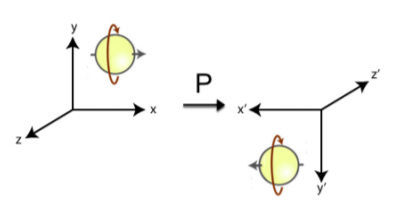
\includegraphics[scale=1]{parity.png}
\centering
\caption{Parity transformation.}
\label{fig:parity}
\end{figure}

True vectors, such as momentum, change sign under the parity transformation, while scalars, such as angular momentum, are invariant. Also under this transformation, scalars, such as energy, remains invariant, while pseudo-scalars, such as helicity, change sign.\\

The parity transformation has also an effect on particles' wave functions. Left-handed particles transform into right-handed particles, and vice-versa, because the spin operator is a pseudo-vector.\\

The ectromagnetic and strong interactions are invariant under the parity transformation, with only the weak interaction violating it.\\

\subsection{Field theory}

For understanding better the effect of the parity transformation, several concepts of field theory have to be introduced.\\

Quantum field theory is a synthesis of quantum mechanics and special relativity. Quantum mechanics is intrinsically a non-relativistic theory, where particles are described by wave functions. When including special relativity, instead of thinking of particles in an external classical potential, one identifies particles with the modes of a field. Thus the Lorentz symmetry is implemented. Particle representations are invariant under the Lorentz transformation and follow a SU(2) symmetry.\\

In this context, we introduce the spinorial representation, one of the fundamental representation of SU(2) group. As such, with spin-1/2 particles it is possible to build composite systems with all possible integer or half-integer spin values.\\

We define the right-handed Weyl spinor, $\psi_R$, and the left-handed Weyl spinor, $\psi_L$, 

\begin{equation}
    \psi_L = (\frac{1}{2},0), 
\end{equation}
\begin{equation}
    \psi_R = (0,\frac{1}{2}).
\end{equation}

We know experimentally that parity is violated by the weak interaction. Theoretically this is reflected by the fact that right- and left-handed components of the spin-1/2 particles enter the theory in a very different way (through the $V-A$ structure). However at sufficiently low energies, the effect of the weak interactions is small. The dominant contributions come from electromagnetic and strong interactions, where parity is conserved. In this case we need to introduce the Dirac field, which provides a representation of the Lorentz and parity transformation,
\begin{equation}
    \Psi = \psi_R = (0,\frac{1}{2}).
\end{equation}

\subsection{V-A structure}

To find out if parity is conserved in an interaction, the parity transformation is applied to the current interaction vertex. For quantum electrodynamics (QED) and quantum chromodynamics (QCD), the form of the interaction vertex is $j^{\mu}=\bar{u}(p')\gamma^{\mu}u(p)$, is that of a vector, so it will change sign under the parity transformation. Since the interaction matrix element is composed of two currents, the negative signs cancel each other and parity is conserved.\\

Due to the fact that weak interaction violates parity, we can assume that the current interaction vertex is not of the same form as that of the QED and QCD currents. The Lorentz invariant requirement restricts the form of the interaction to covariant bilinear combinations of two spinors. The most general form for the interaction between a boson and a fermion with the exchange of a spin-1 boson is a linear combination of vector and axial vector currents, 
\begin{equation}
    j^{\mu} \propto g_V j^{\mu}_V + g_A j^{\mu}_A, 
\end{equation}

where $g_v$ and $g_A$ are vector and axial vector coupling constants, respectively. Thus, the weak interaction has two components. One violates parity and the other conserves parity. The relative strength of the parity violating part compared to the parity conserving part is given by

\begin{equation}
    \alpha = \frac{g_V \cdot g_A}{g^2_V + g^2_A}.
\end{equation}

If one of the coupling constants is zero, parity is conserved. Maximal parity violation happens when $|g_V|=|g_A|$. Experiments confirm that the structure of the weak charged current is a vector minus the axial vector ($V-A$), with this vertex factor being given by
\begin{equation}
    \frac{- i g_W}{\sqrt{2}}\frac{1}{2}\gamma^{\mu}(1-\gamma^5).
\end{equation}

\subsection{Fermi theory}

The weak interactions are mediated by the massive boson $W^+$, $W^-$ and $Z^0$. Since the $W^{\pm}$ bosons are electrically charged, only they can exchange charge via the charge current interaction, as well as the quark flavour, as illustrated in Figure~\ref{fig:WInteraction}.
  
\begin{figure}[h]
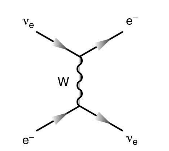
\includegraphics[scale=0.8]{charged.png}
\centering
\caption{Feynman Diagram for the charged current interaction.}
\label{fig:WInteraction}
\end{figure}  
  
Let's considere the interaction Lagrangian for the weak charged interactions
\begin{equation}
    L_{\rm CC} = g_W(W^+_{\mu}J^{+ ,\mu} + W^-_{\mu}J^{- ,\mu}),
\end{equation}

where the charge-raising current operator and the charge-lowering operator are given by
\begin{equation}
    J^+ = \frac{1}{\sqrt{2}} \sum_l (\bar{\nu_l}\frac{\gamma^{\mu}(1-\gamma^5)}{2}l) + \sum_q (\bar{q'}\frac{\gamma^{\mu}(1-\gamma^5)}{2}q),
\end{equation}

\begin{equation}
    J^- = \frac{1}{\sqrt{2}} \sum_l (\bar{l}\frac{\gamma^{\mu}(1-\gamma^5)}{2}\nu_l) + \sum_q (\bar{q}\frac{\gamma^{\mu}(1-\gamma^5)}{2}q').
\end{equation}

The sum over $l$ is the sum over the leptons, and the sum over $q$ is the sum over the quarks, where $q=(u,c,t)$ are the quark mass eigenstates and $q'=(d',s',b')$ are the flavor eigenstates, which are also the weak interaction eigenstates of the Cabbibo-Kobayashi-Maskawa matrix.\\

The $Z^0$ boson is neutral (no electric charge). Thus it is the mediator of neutral current interaction, as illustrated in the Figure~\ref{fig:ZInteraction}. The interaction Lagrangian for the weak neutral interactions is given by
\begin{equation}
    L_{\rm NC} = \frac{g_W}{\cos{\theta_W}}J^{\mu}_Z Z_{\mu}.
\end{equation}

\begin{figure}[h]
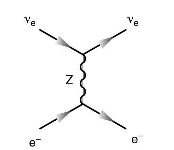
\includegraphics[scale=0.8]{neutral.png}
\centering
\caption{Feynman Diagram for neutral current interaction.}
\label{fig:ZInteraction}
\end{figure}  

Thus the neutral current is
\begin{equation}
    J_Z = \sum_j \bar{\psi_j}\gamma^{\mu} (\frac{(1-\gamma^5)}{2}T^3 - 2\sin^2{\theta_W}Q_j), 
\end{equation}

where the $T^3$ and Q are the weak isospin and the charge of the particle, respectively. $\theta_W$ represents the rotation due to the spontaneous symmetry breaking, or in other words thus the angle between the particles that are mass eigenvalues and the ones that are weak eigenvalues.\\

We take into consideration both the charged current (CC) and neutral current (NC), whose invariant amplitudes are given by
\begin{equation}
    i M_{\rm CC} = (-i g_W)^2 J^{\mu}_+ [\frac{-i}{q^2-M^2_W}(\eta_{\mu\nu}-\frac{q_{\mu}q_{\nu}}{M^2_W})] J_{- \mu},
\end{equation}
\begin{equation}
    i M_{\rm NC} = (\frac{-i g_W}{\cos{\theta_W}})^2 J^{\mu}_Z [\frac{-i}{q^2-M^2_z}(\eta_{\mu\nu}-\frac{q_{\mu}q_{\nu}}{M^2_z})] J_{Z \mu}.
\end{equation}

Nevertheless, most of the interactions take places at low energies (on the order of a few \GeV). Since the mass of the boson dominates the kinematics of the propagator, we can assume the approximation $|q^2| << M^2_W$, which allows to describe weak interactions as an effective theory, and to express the $W$-boson propagator as

\begin{equation}
    \frac{-i}{q^2-M^2_W}(\eta_{\mu\nu}-\frac{q_{\mu}q_{\nu}}{M^2_W}) \rightarrow \frac{i \eta_{\mu\nu}}{M^2_W}.
\end{equation}

The effective interaction has no longer a $q$ dependence. Physically this corresponds to replacing the propagator with an interaction which occurs at a single point in space-time, or in other words with a point-like interaction, as illustrated in Figure~\ref{fig:PointLikeInteraction}.

\begin{figure}[h]
\includegraphics[scale=0.5]{Fermi.png}
\centering
\caption{Point like interaction.}
\label{fig:PointLikeInteraction}
\end{figure}  

For a general leptonic interaction the invariant amplitude is reduced to
\begin{equation}
    i M_{\rm CC} = \frac{- i g_W^2}{8M_W^2}[\bar{\nu_l}\gamma^{\mu}(1-\gamma^5)l][\bar{l}\gamma^{\mu}(1-\gamma^5)\nu_l], 
\end{equation}

where the relation between the weak interaction coupling constant and the coupling Fermi constant is given by
\begin{equation}
    \frac{G_F}{\sqrt{2}} = \frac{g_W^2}{8 M_W^2}.
\end{equation} 

Therefore, the interaction term in the effective theory Lagrangian is given by
\begin{equation}
L = \frac{-G_F}{\sqrt{2}}(j^{+,\mu} j^-_{\mu}),
\end{equation}

where $j = 2\sqrt{2} J$.

\subsection{$\beta$ disintegration}

In this experiment, we use a radioactive source that produces electrons via nuclear beta  ($\beta$) disintegration, where one neutron transforms to one proton. In order to study the parity violation in this process, the effective theory is used, considering that in this case the energies involved are smaller than the masses of the particles. However is not easy to compute the invariant amplitude, since the particles are not free. Nucleons (neutrons and protons) are bound states of quarks. Quarks create a field consisting on gluons. So it is also necessary to consider the vacuum fluctuations that create pairs of quarks and antiquarks.

\section{Moller Diffusion}

The experiment is based on sending the electrons coming from the source onto an iron target. The incident electrons are scattered off by the atoms and electrons of the target. But we are only interested in the following reaction
\begin{equation}
    e^- + e^- \rightarrow e^- + e^-.
\end{equation}

This process is described by four tree-level diagrams (neutral current): the two from QED, exchanging a photon ($\gamma$) and an identical pair in which a $Z$ boson is exchanged, as illustrated in Figure~\ref{fig:MollerScattering}. The weak force is purely left-handed, but the weak and electromagnetic forces mix into the particles we observe, 

\begin{figure}[h]
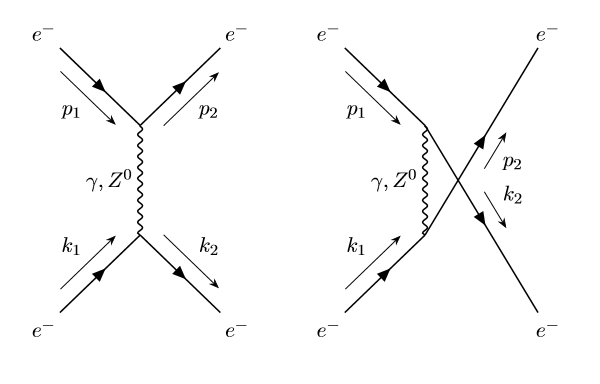
\includegraphics[scale=0.5]{moller.png}
\centering
\caption{t-channel and u-channel Feynman diagrams for the Moller scattering.}
\label{fig:MollerScattering}
\end{figure}

The photon is symmetric by construction, but the $Z$ boson prefers left-handed particles to right-handed particles. Thus the cross sections for left-handed electrons and right-handed differ.  The invariant amplitude of this process is given by

\begin{multline}
\\
     i\mathcal{M} = i\mathcal{M}^{\gamma}_{\rm t-channel} + i\mathcal{M}^{\gamma}_{\rm u-channel} + i\mathcal{M}^{Z}_{\rm t-channel} + i\mathcal{M}^{Z}_{\rm u-channel} =\\ [\bar{u}(k_2)(-ie\gamma^{\mu})u(k_1)][\frac{-i\eta_{\mu\nu}}{(k_1-k_2)^2}][\bar{u}(p_2)(-ie\gamma^{\nu})u(p_1)] -\\
    [\bar{u}(p_2)(-ie\gamma^{\mu})u(k_1)][\frac{-i\eta_{\mu\nu}}{(k_1-p_2)^2}][\bar{u}(k_2)(-ie\gamma^{\nu})u(p_1)] +\\
    (-i \frac{g_W}{\cos{\theta_W}})^2[\bar{u}(k_2)\frac{(\gamma^{\mu}(c_v - c_A\gamma^5)}{2}u(k_1)][\frac{-i(\eta_{\mu\nu}-\frac{(k_1-k_2)_{\mu}(k_1-k_2)_{\nu}}{M_Z^2})}{(k_1-k_2)^2-M_Z^2}][\bar{u}(p_2)\frac{(\gamma^{\mu}(c_v - c_A\gamma^5)}{2}u(p_1)] -\\
    (-i \frac{g_W}{\cos{\theta_W}})^2[\bar{u}(p_2)\frac{(\gamma^{\mu}(c_v - c_A\gamma^5)}{2}u(k_1)][\frac{-i(\eta_{\mu\nu}-\frac{(k_1-p_2)_{\mu}(k_1-k_2)_{\nu}}{M_Z^2})}{(k_1-k_2)^2-M_Z^2}][\bar{u}(k_2)\frac{(\gamma^{\mu}(c_v - c_A\gamma^5)}{2}u(p_1)].
\end{multline}

The maximum energy of the electrons emitted by the strontium-90 source is 2.28 MeV, which falls in the low energy range. Thus it is acceptable to neglect the process due to the weak interaction, and the invariant amplitude becomes

\begin{multline}
     i\mathcal{M} = [\bar{u}(k_2)(-ie\gamma^{\mu})u(k_1)][\frac{-i\eta_{\mu\nu}}{(k_1-k_2)^2}][\bar{u}(p_2)(-ie\gamma^{\nu})u(p_1)] -
    [\bar{u}(p_2)(-ie\gamma^{\mu})u(k_1)][\frac{-i\eta_{\mu\nu}}{(k_1-p_2)^2}][\bar{u}(k_2)(-ie\gamma^{\nu})u(p_1)] .
\end{multline}

Once the invariant amplitude is known, we can compute the cross section, which in the centre-of-mass is defined as

\begin{equation}
    \frac{d\sigma}{d\Omega} = \frac{1}{\pi^2}\frac{E_1^2E_2^2}{(E_1+E_2)^2} \sum_{\rm spins} |\mathcal{M}|^2.
\end{equation}

We have to sum over all the spins in the final state, because we accept all the possible configurations. For the initial state we know the spin configurations of the electrons coming from the source. 

\subsection{Polarisation}

Since the process is a $\beta$ disintegration, the electrons are left-handed due to weak interaction structure. Thus they are longitudinally polarised.\\

The electrons from the target are in the external orbitals. When this target is placed inside a magnetic field, their spins of the electrons of the target are aligned with the field, so the electrons are longitudinal polarised.\\

Since both electrons are longitudinal polarised, we can have two different cross sections for the different spin configuration: parallel ($\sigma_{\leftleftarrows}$) or antiparallel ($\sigma_{\rightleftarrows}$) polarisation.\\

For describing the longitudinal polarisation, it is necessary to impose that the spinors $u_{\epsilon1}$ and $u_{\epsilon2}$ are eigenstates of the spin operator $\frac{1}{2}\Sigma = \sigma \frac{p}{|p|}$, such that

\begin{equation}
\frac{1}{2}
   \begin{pmatrix}
   \vec{\sigma} && 0 \\
   0 && \vec{\sigma}
   \end{pmatrix} \cdot u_{\epsilon} = \epsilon \cdot u_{\epsilon} \quad \Rightarrow \quad \begin{matrix} u_{\epsilon 1} = \frac{1}{2} \Sigma_{\epsilon} (1+\epsilon_1 \sigma_1) u_{\epsilon}\\
   u_{\epsilon 2} = \frac{1}{2} \Sigma_{\epsilon} (1+\epsilon_2 \sigma_2) u_{\epsilon}
   \end{matrix}.
\end{equation}

Using the completeness relation ($\sum_{s=1,2} u^{(s)}(p) \bar{u}^{(s)}(p) =  \displaystyle{\not} p + m
$) and the notation above, we define the cross section as
\begin{equation}
    \frac{d\sigma}{d\Omega} = \frac{\alpha^2 E_1^2E_2^2}{(E_1+E_2)^2 E_1'E_2'} (\frac{\rm A}{(k_1 - k_2)^2} + \frac{\rm B}{(k_1 - p_2)^2} - \frac{\rm C+D}{(k_1 - k_2)^2(k_1 - p_2)^2}),
\end{equation}

where $\alpha$ is the fine structure constant, defined as $e^2/4\pi$. Also A and B are defined as 

\centerline{${\rm A} =  \frac{1}{16} Tr[(k_1+im_e)\gamma_{\mu}(1+\epsilon_1\sigma_{k1})(k_2+im_e)\gamma_{\nu}(p_1+im_e)\gamma^{\mu}(1+\epsilon_2\sigma_{p1})(p_2+im_e)\gamma^{\nu}]$,}

\centerline{${\rm B} = \frac{1}{16} Tr[(k_1+im_e)\gamma_{\mu}(1+\epsilon_1\sigma_{k1})(p_2+im_e)\gamma_{\nu}(p_1+im_e)\gamma^{\mu}(1+\epsilon_2\sigma_{p1})(k_2+im_e)\gamma^{\nu}]$,}

respectively. Furthermore, C and D are obtained from A and B, respectively, by exchanging $k_1$ for $p_1$.\\

We define the cross section with parallel and antiparallel initial spins, respectively, as illustrated in Figure~\ref{fig:ParallelAntiparallelPolarisation}.

\begin{figure}[h]
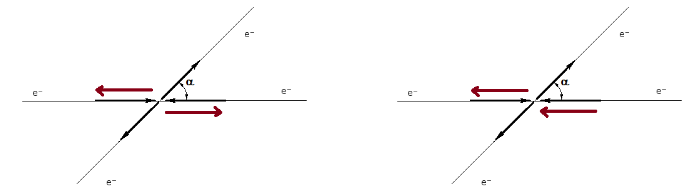
\includegraphics[scale=0.5]{polarisation.png}
\centering
\caption{Parallel and antiparallel polarisation.}
\label{fig:ParallelAntiparallelPolarisation}
\end{figure}

This implies that \\
        \centerline{parallel spins $\rightarrow \epsilon_1 = - \epsilon_2$, }\\
        \centerline{antiparallel spins $\rightarrow \epsilon_1 = \epsilon_2$.}
        
 Developing the traces and using the previous relation, in the centre-of-mass we obtain the following cross sections
 \begin{equation}
     \sigma_{\leftleftarrows} = \alpha^2 \frac{2\cos^2{\theta}+\beta^2(3\cos^2{\theta}+\cos^4{\theta})+\beta^4(1+\cos^4{\theta})}{2E^2\beta^4\sin^2{\theta}},
 \end{equation}
 
 \begin{equation}
     \sigma_{\rightleftarrows} = \alpha^2 \frac{1+\cos^2{\theta}+\beta^2(2+3\cos^2{\theta}-\cos^4{\theta})+\beta^4(5-4\cos^2{\theta}+\cos^4{\theta})}{2E^2\beta^4\sin^2{\theta}},
 \end{equation}
 
where $\beta$ is the ratio of the velocity and the speed of light, $\gamma$ is the Lorentz factor and $\theta$ is the diffusion angle.

\subsection{Asymmetry}
\label{asym}

By the definition of the cross section, it would be possible to measure it experimentally by
\begin{equation}
    \sigma = \frac{N}{L \epsilon A}.
\end{equation}

We know the flux ($N$), but we do not know the luminosity ($L$), the efficiency ($\epsilon$), and the acceptance of the detector ($A$). Since it is impossible to measure the cross section in this experiment, we are interested in the asymmetry, defined as
\begin{equation}\label{27}
    A = \frac{\sigma_{\rightleftarrows}-\sigma_{\leftleftarrows}}{\sigma_{\rightleftarrows}+\sigma_{\leftleftarrows}} = \frac{1-\cos^2{\theta}+\beta^2(2-2\cos^4{\theta})+\beta^4(4-5\cos^2{\theta}+\cos^4{\theta})}{1+3\cos^2{\theta}+\beta^2(2+6\cos^2{\theta})+\beta^4(6-3\cos^2{\theta}+\cos^4{\theta})}.
\end{equation}

We can see in Figure~\ref{fig:angle} the cross section as a function of the angle with $\beta=1$, which means that the energy is also fixed. We observe that the asymmetry is maximal when the angle is $\pi/2$.

\begin{figure}[H]
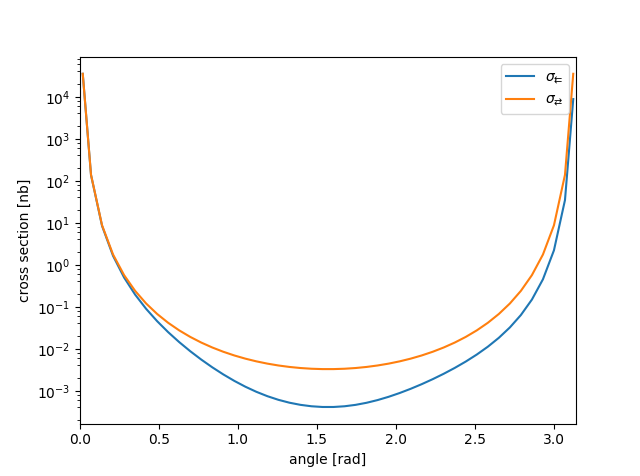
\includegraphics[scale=0.5]{angle.png}
\centering
\caption{Cross section as function of the angle with $\beta = 1$.}
\label{fig:angle}
\end{figure}

In Figure~\ref{fig:energy} it is represented the cross section as a function of the energy, with $\theta=\pi/2$ and $\beta=1$.

\begin{figure}[H]
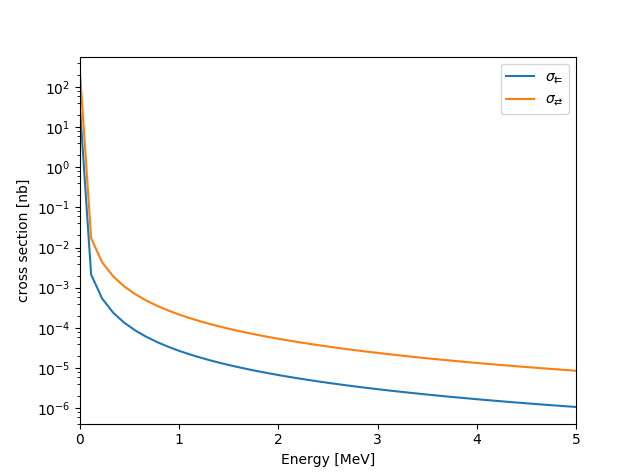
\includegraphics[scale=0.5]{energy.png}
\centering
\caption{Cross section as a function of the energy with $\theta=\pi/2$.}
\label{fig:energy}
\end{figure}

We can also represent the asymmetry for the fixed angle $\theta=\pi/2$ that makes the asymmetry maximal, as a function of the the ratio of the velocity and the speed of light, $\beta$, as illustrated in Figure~\ref{fig:asymmetry}.

\begin{figure}[H]
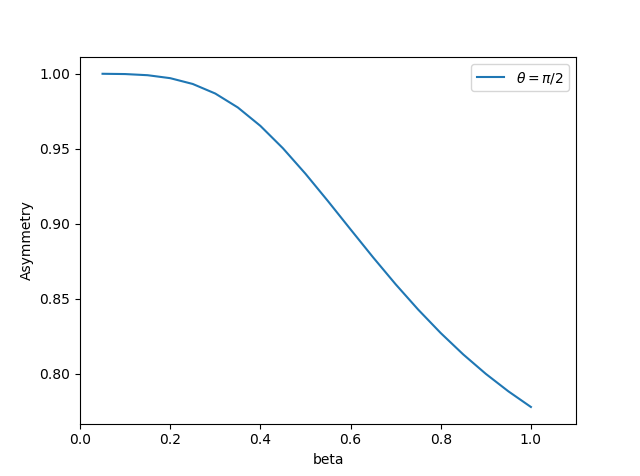
\includegraphics[scale=0.5]{asym.png}
\centering
\caption{Asymmetry as a function of $\beta$ with $\theta=\pi/2$.}
\label{fig:asymmetry}
\end{figure}

In this experiment, we are not measuring the asymmetry, but the number of electrons arriving to the detectors. Thus, finding the relation between the asymmetry of cross sections and the count rate of the detectors is crucial.\\

Some of the electrons detected have no correlation between their polarisations. Therefore we have to define the cross section of unpolarised electrons, $\sigma_0 = 1/2 (\sigma_{\leftleftarrows} + \sigma_{\rightleftarrows})$.\\

Denoting $P_{\rm s}$ as the longitudinal polarisation of the electrons emitted by the source and $P_{\rm t}$ the longitudinal polarisation of the electrons in the target, we can define the count rate for the electrons with parallel polarisation ($C_{\leftleftarrows}$) and antiparallel polarisation ($C_{\rightleftarrows}$) as

\begin{equation}\label{28}
C_{\leftleftarrows} \approxeq P_{\rm s} P_{\rm t} \sigma_{\leftleftarrows} + (1-P_{\rm s} P_{\rm t})\sigma_0,
\end{equation}
\begin{equation}
C_{\rightleftarrows} \approxeq P_{\rm s} P_{\rm t} \sigma_{\rightleftarrows} + (1-P_{\rm s} P_{\rm t})\sigma_0.
\end{equation}

Using the previous relations we can define as well the count rate of the asymmetry as

\begin{equation}\label{30}
\epsilon=\frac{C_{\rightleftarrows}-C_{\leftleftarrows}}{C_{\rightleftarrows}+C_{\leftleftarrows}} \approxeq P_{\rm s} P_{\rm t} \frac{\sigma_{\rightleftarrows}-\sigma_{\leftleftarrows}}{\sigma_{\rightleftarrows}+\sigma_{\leftleftarrows}}= P_{\rm s} P_{\rm t} \cdot A(\theta,\beta).
\end{equation}

In this way we succeed in relating the cross section with experimental observables, the asymmetry in the counting rate and the polarisation of the electrons.

\section{Kinematics}

In this section the relation between the centre-of-mass (c.o.m or com) angle and the laboratory angle will be computed, so we can show that the positions of the detectors are fixed to maximise the value of the asymmetry.\\

As the interaction is at low energy we can consider it as an elastic collision, as illustrated in Figure~\ref{fig:lab}.
\begin{figure}[H]
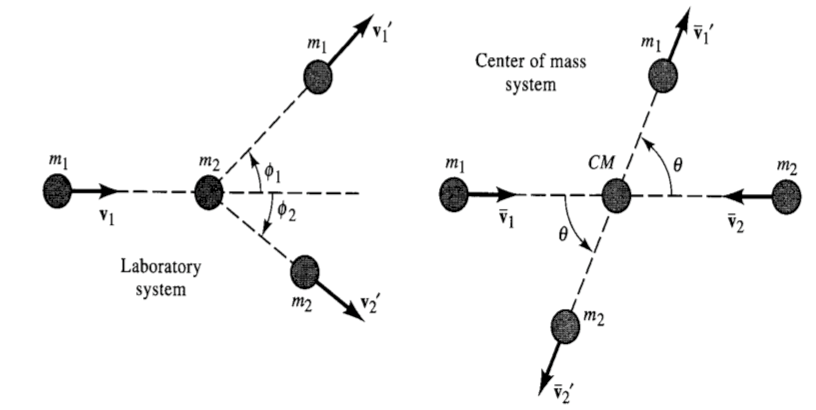
\includegraphics[scale=0.3]{lab.png}
\centering
\caption{Comparison between the lab (left) and c.o.m (right) reference frames.}
\label{fig:lab}
\end{figure}

With the initial quadri-vectors (4-vectors) we can define

\begin{equation}
    P^{\mu}_{\rm lab,1} = (E_{\rm lab,1},p_{\rm lab,1},0,0)
\end{equation}

\begin{equation}
    P^{\mu}_{\rm lab,2} = (m_e,0,0,0)
\end{equation}

\begin{equation}
    P^{\mu}_{\rm com,1} = (E_{\rm com,1},p_{\rm com,1},0,0)
\end{equation}

\begin{equation}
    P^{\mu}_{\rm com,2} = (E_{\rm com,2},-p_{\rm com,1},0,0)
\end{equation}

After the collision, using energy conservation and the fact that the norm of the 4-vectors are equals, $P^{\mu}_{\rm com,3} = (E_{\rm com,1},p_{\rm com,1}\cos{\theta_{\rm com}},p_{\rm com,1}\sin{\theta_{\rm com}})$, we can perform a Lorentz transformation to obtain the 4-vector in the lab frame as

\begin{equation}
P^{\mu}_{\rm lab,3} = \begin{pmatrix}
\gamma & \gamma\beta & 0 & 0 \\
\gamma\beta & \gamma & 0 & 0\\
0 & 0 & 1 & 0\\
0 & 0 & 0 & 1
\end{pmatrix};
P^{\mu}_{\rm com,3} = \begin{pmatrix}
\gamma[E_{\rm com,1}+\beta p_{\rm com,1}\cos{\theta_{\rm com}}]\\
\gamma[\beta E_{\rm com,1}+ p_{\rm com,1}\cos{\theta_{\rm com}}]\\
p_{\rm com,1}\sin{\theta_{\rm com}}]\\
0
\end{pmatrix}.
\end{equation}

By looking at Figure~\ref{fig:lab} we can find a relation for the angle in the lab frame

\begin{equation}\label{eq:2}
    \tan{\theta_{\rm lab}} = \frac{P^y_{\rm lab,3}}{P^x_{\rm lab,3}} = \frac{\sin{\theta_{\rm com}}}{\gamma(\cos{\theta_{\rm com}}+\frac{\beta E_{\rm com,1}}{p_{\rm com,1}})}.
\end{equation}

For solving this equation first of all, we will focus on the energy and momentum of the c.o.m term, which by using a Lorentz transformation we can express as

\begin{equation}\label{eq:3}
    \frac{\beta E_{\rm com,1}}{p_{\rm com,1}} = \frac{\beta (E_{\rm lab,1}-\beta p_{\rm lab,1})}{p_{\rm lab,1}-\beta E_{\rm lab,1}}.
\end{equation}

In the centre-of-mass the speed of the particle can be expressed as $v_{\rm com,1} = \frac{p_{\rm com,1}}{E_{\rm com,1}}$, where $v_{\rm com,1} = \beta_{\rm com,1}$. Using this relation we can set the equivalence

\begin{equation}\label{eq:4}
    \frac{\beta E_{\rm com,1}}{p_{\rm com,1}} = \frac{\beta}{\beta_{\rm com,1}}.
\end{equation}

By imposing that $P^x_{\rm lab,1}=-P^x_{\rm lab,2}$, we are lead to the expression
\begin{equation}\label{eq:1}
    \beta = \frac{p_{\rm lab,1}}{E_{\rm lab,1}+m_e}.
\end{equation}

By also using the relation $E_{\rm lab,1}=E_{\rm kinetic}+m_e$ we find 

\begin{equation}\label{eq:5}
    \frac{\beta}{\beta_{\rm com,1}} = 1.
\end{equation}

From Equation \ref{eq:1} we can rewrite the Lorentz factor as
\begin{equation}\label{eq:6}
    \gamma = \frac{1}{\sqrt{1-\beta^2}}= \frac{E_{\rm kinetic}+m_e}{\sqrt{4m_e^2 + 2 E_{\rm kinetic}m_e}}.
\end{equation}

As explained in the previous section, we obtain the maximal relation for an angle $\theta_{\rm com} = \pi/2$, but the angle in the laboratory frame is not the same, as we can see from Equation \ref{eq:2}. By using the Equations \ref{eq:4}, \ref{eq:5} and \ref{eq:6}, we determine the angle in the laboratory frame as

\begin{equation}
    \tan{\theta_{\rm lab}}= \frac{1}{\gamma}\frac{\sin{(\pi/2)}}{\cos{(\pi/2)}+1} = \frac{1}{\gamma} = \frac{\sqrt{4m_e^2 + 2 E_{\rm kinetic}m_e}}{E_{\rm kinetic}+2m_e}.
\end{equation}

\begin{figure}[h]
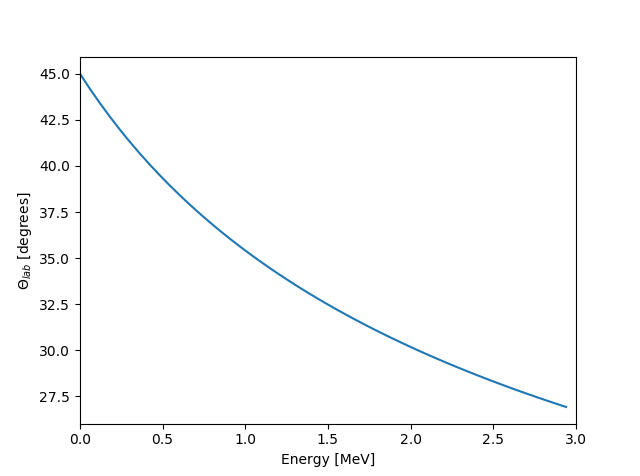
\includegraphics[scale=0.5]{theta.png}
\centering
\caption{Diffusion angle in the lab as a function of the incident energy.}
\label{fig:theta}
\end{figure}

In Figure \ref{fig:theta} we can see the scattering angle in the lab frame as a function of the incident particle at a fixed angle in the centre-of-mass.\\

Since the Yttrium-90 source is disintegrated with an average energy of 0.933 \MeV~and a maximal energy of 2.28 \MeV, we can say that the electrons will be scattered with angles around 36 and 29 degrees. Thus, we fixed the detectors at $35 \pm 11$ degrees. In this way, we maximise the possibilities of detecting most of the events. \\

We assume that the incident electron gives half of its kinetic energy to the electron in the target. This implies that the exiting electron has half of the incoming energy,  or $E_{\rm outgoing} = E/2$. This relation will be fundamental in the data analysis in order to select events with energy compatible with the experimental setup.

\chapter{Experimental setup}

\section{Setup}
\begin{figure}[h]
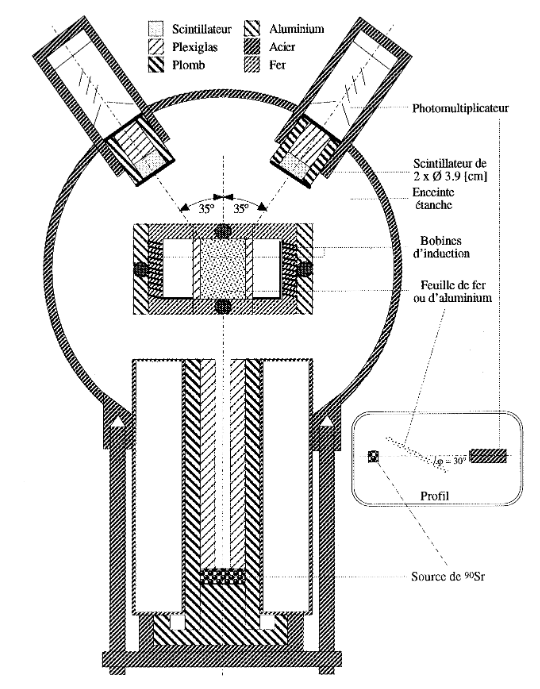
\includegraphics[scale=0.5]{setup.png}
\centering
\caption{Schema of the experimental setup.}
\label{fig:setup}
\end{figure}

Figure \ref{fig:setup} illustrates an overview of the experimental setup. For this experiment we are using as a $\beta$ emitter a Strontium-90 source, which is located in the lower part of the schema. It is surrounded by lead to avoid the radiation goes outside. The source is facing an enclosure of around 35 cm of diameter that can be closed with a lid, which is made of the same material as the enclosure, namely steel.\\

Oriented at an angle of $35 \pm 11$ degrees, as mentioned before, in the right and left sides of the target there are two plastic scintillators, each one coupled to a light guide and a photomultiplier. The electrons coming from the Moller scattering off the target lose energy when traversing the scintillator, which leads to an excitation of its molecules. The excited molecules from the scintillator tends to find their minimum energy by losing this excess energy in the form of emitted photons, which are guided through the photomultipliers by the guide lights.\\

An image of the physical setup is illustrated in Figure~\ref{fig:setupexp}.

\begin{figure}[h]
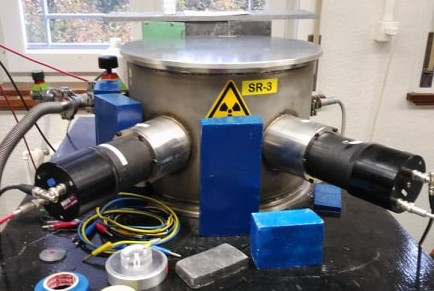
\includegraphics[scale=0.8]{experimentalsetup.jpg}
\centering
\caption{Actual image of the experimental setup.}
\label{fig:setupexp}
\end{figure}

In the middle of the enclosure there is the support where the target is fixed, namely an aluminium or iron target, as well as the induction coils, as seen in Figure \ref{fig:cible}).

\begin{figure}[H]
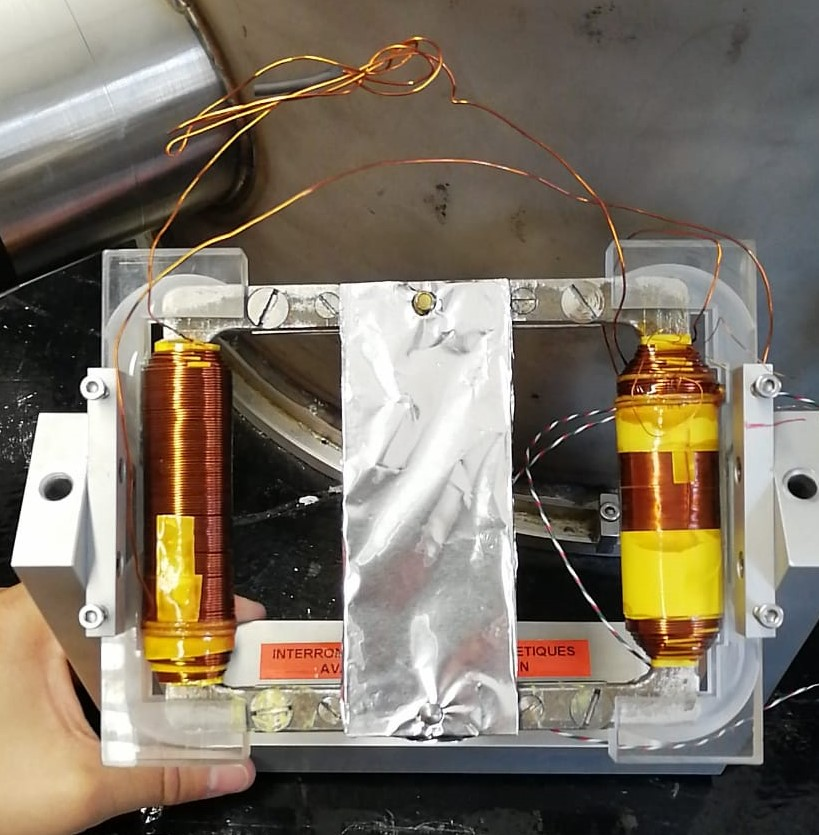
\includegraphics[scale=0.3]{cible.jpeg}
\centering
\caption{Actual image of the target.}
\label{fig:cible}
\end{figure}

The incident electrons coming from the source are interacting with the electrons in the target via Moller scattering. As said in the previous section, the electrons coming from the source are right-handed and have a longitudinal polarisation. Thanks to the coils, we can control the magnetic field applied to the target. Therefore we can control the polarisation of the electrons in the target, making them either parallel or antiparallel relative to the ones coming from the source. An iron foil is used as a target given its ferromagnetic properties. We can then change the orientation of all the spins in the target, using a low magnetic field. \\

All the components are placed in vacuum, at approximately 1.8 mbar, in order to minimise the electron energy lost and multiple scattering with air particles.

\section{Radioactive Source}

The source used in this experiment is Strontium-90 ($\prescript{90}{38}{\mathbf{Sr}}$). It disintegrate into Yttrium-90 ($\prescript{90}{39}{\mathbf{Y}}$) via the $\beta$-decay, which produces one electron and one electron antineutrino, with a half-life of 28.79 years. This is the only channel of disintegration and is described by

 \begin{equation}
     \prescript{90}{38}{\mathbf{Sr}} \rightarrow \prescript{90}{39}{\mathbf{Y}} + e^- +\bar{\nu}_e.
 \end{equation}
 
 In turn, Yttrium-90 decays with a half-time of 64 hours via the $\beta$-decay into Zirconium-90 ($\prescript{90}{40}{\mathbf{Zr}}$), creating again, another electron and another electron antineutrino, as given by
 
\begin{equation}
     \prescript{90}{39}{\mathbf{Y}} \rightarrow \prescript{90}{40}{\mathbf{Zr}} + e^- +\bar{\nu}_e .
 \end{equation}

The energy of the electrons released during the first disintegration is on average of 0.196 \MeV, with a maximum value of 0.927 \MeV. For the second disintegration the average energy released by the electron is 0.927 \MeV, with a maximum energy of 2.28 \MeV. The chain of the two radioactive decays are illustrated in Figure~\ref{fig:Sr90}. As discussed before, the electrons measured in this experiment are the ones coming from the second disintegration. This fact will be an automatic consequence due to the energy range used to treat the data, as described in the following chapter.

\begin{figure}[H]
\includegraphics[scale=0.5]{Sr90.jpg}
\centering
\caption{Strontium-90 decay diagram.}
\label{fig:Sr90}
\end{figure}

\section{Photomultiplier tube}

A photomultiplier tube (PMT) is a detector sensible to light, widely use in high energy physics. As illustrated in Figure \ref{fig:PMT}, a PMT consists of a photocathode, a chain of dynodes and an anode. The photocathode is negatively charged and recoated with a material capable of releasing an electron as soon as a photon arrives, due to the photoelectric effect. A dynode is an electrode in a vacuum tube that serves as an electron multiplier through secondary emission.

\begin{figure}[H]
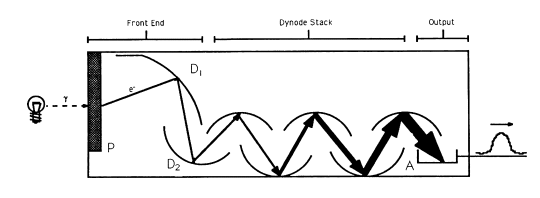
\includegraphics[scale=0.5]{PMT.png}
\centering
\caption{Schematic of a Photomultiplier tube.}
\label{fig:PMT}
\end{figure}

As said before, the electrons emitted from the cathode are accelerated toward the first dynode. Each accelerated photoelectron that strikes the dynode surface frees several electrons from the surface. These electrons are then accelerated toward the second dynode, held more positive than the first dynode. Each electron that strikes the surface of the second dynode produces several more electrons, which are then accelerated toward the third dynode, and so on. The final result is producing an avalanche, thus a multiplication of the signal.\\

The photomultipliers tubes used in this experiment are manufactured by Hamamatsu. They have with a diameter of 5.1cm and contain a photo-sensible surface of a diameter of 4.6 cm. The gain, or ratio between the secondary electrons between two dynodes, increases linearly with the applied voltage.
In order to chose the optimised value for the tension applied to the PMT, a calibration is needed, as discussed in Section~\ref{sec:Calibration}.

\section{Electronics}

This amplified signal arrives to the electronics. Its schematic treatment there is illustrated in Figure~\ref{fig:electronicsSchema}, while the actual image of the electronics of the experiment is presented in Figure~\ref{fig:electronicsActual}.

\begin{figure}[H]
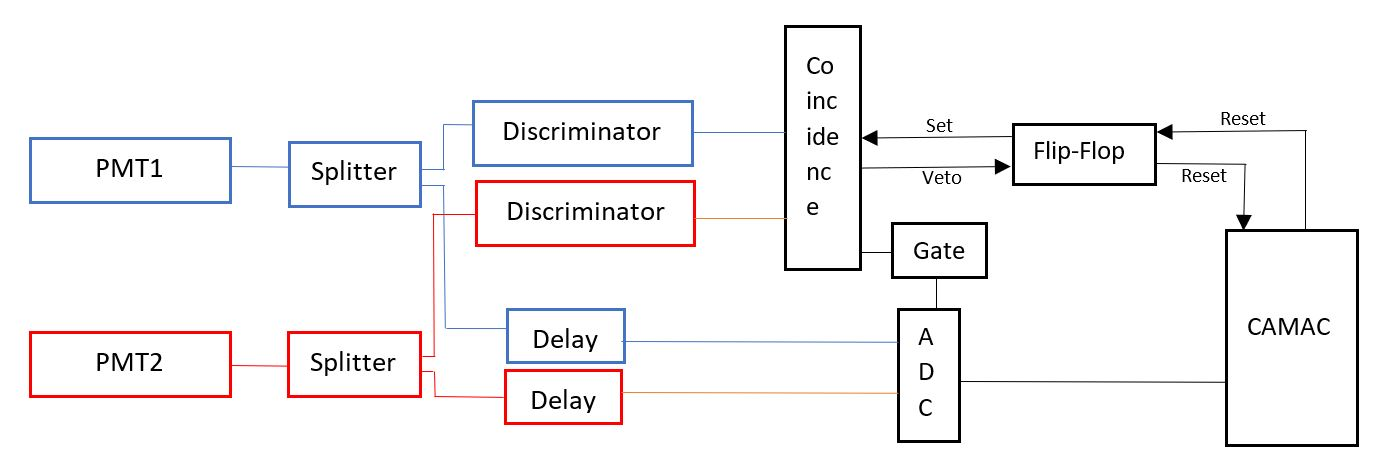
\includegraphics[scale=0.5]{electronics.JPG}
\centering
\caption{Schema of the electronics}
\label{fig:electronicsSchema}
\end{figure}

The signal coming from the PMT goes to a splitter, which divides the signal in two. \\

One of the two outputs is connected to a discriminator. It converts the analog signal into a digital one, with a fixed width and threshold, which only allows certain values of the signal.\\

The output of both discriminators goes to the coincidence device, which works as a trigger. When the signals coming from PMT1 and PMT2 are synchronised, the coincidence signal splits in two. One part of the signal goes to a flip-flop module, which is connected to the CAMAC. The veto, coming from the coincidence, avoids the trigger to act again.\\

The other part of the signal goes to a gate, that represents the window in which the ADC module is acquiring data coming from the PMTs after passing through a delay. This delay is needed to ensure that the signals coming from the PMT arrives to the ADC in the acquiring window set by the gate.\\

This process avoids the overlap between different events. Thus there is a dead time, during which the system is not acquiring new data. During this time, the ADC is converting the signal into binary data. The CAMAC will read this data and send it to the computer where it will be stored. Once the data is read, the CAMAC restarts the flip-flop and new data can be acquired.

\begin{figure}[H]
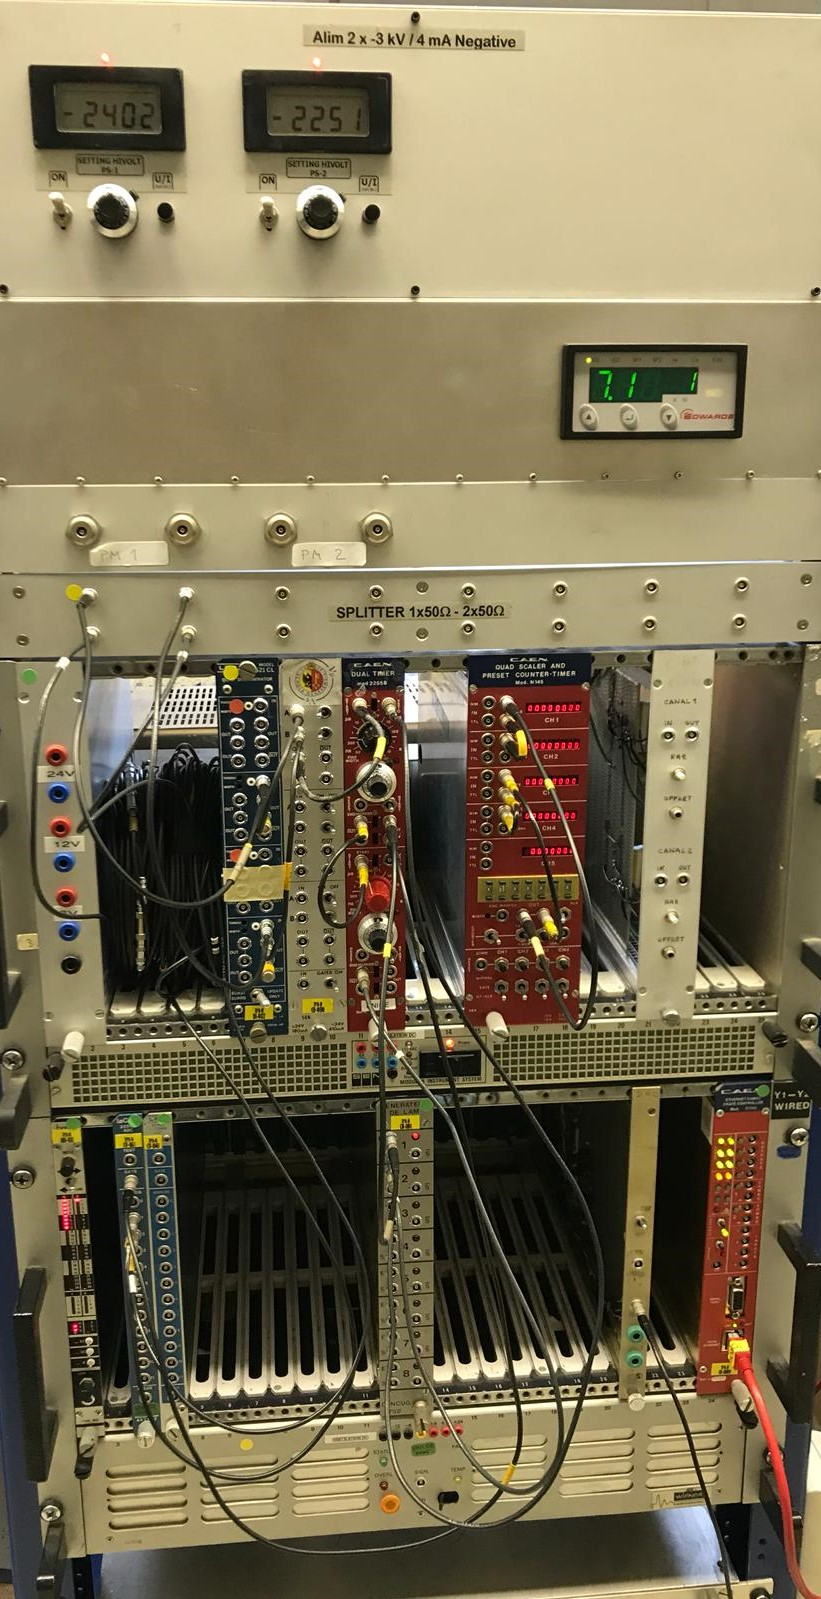
\includegraphics[scale=0.3]{electronics.jpeg}
\centering
\caption{Actual image of the electronics of the experiment.}
\label{fig:electronicsActual}
\end{figure}

\chapter{Calibration and measurements}
\label{sec:Calibration}

The formal definition of calibration by the BIPM is ``operation that, under specified conditions, in a first step establishes a relation between the quantity values with measurement uncertainties provided by measurement standards and corresponding indications with associated measurement uncertainties and, in a second step, uses this information to establish a relation for obtaining a measurement result from an indication.'' Therefore the calibration of the PMTs used in this experiment is crucial.

\section{Calibration}

We need to determine the optimal working regime of the PMTs in our experiment. We need to focus mainly in the linearity, the resolution, the coincidence tax and the energy. For doing this calibration we use a source of $\prescript{207}{}{Bi}$ and make measurements of its spectrum for different voltages. The Figure~\ref{fig:spectrum} presents the spectrum of the source measured by the PMT2 at 2100 V.

\begin{figure}[H]
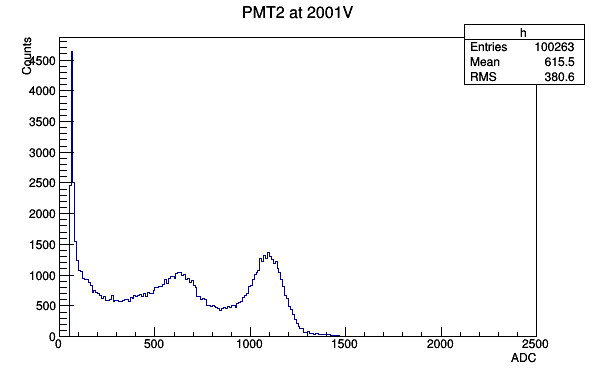
\includegraphics[scale=0.7]{spectrum.png}
\centering
\caption{Mean as a function of the voltage for both PMT}
\label{fig:spectrum}
\end{figure}

We observe two peaks. The left one is due to the Strontium and the right one is due to the Bismuth. For assuring the linearity of the PMTs in the voltage range, we need to fit the second peak (Bismuth) and compute the mean of the Gaussian fit for each voltage. The figure \ref{fig:mean} show the variation of the mean as a function of the voltage, which validates the linearity of the PMTs.

\begin{figure}[H]
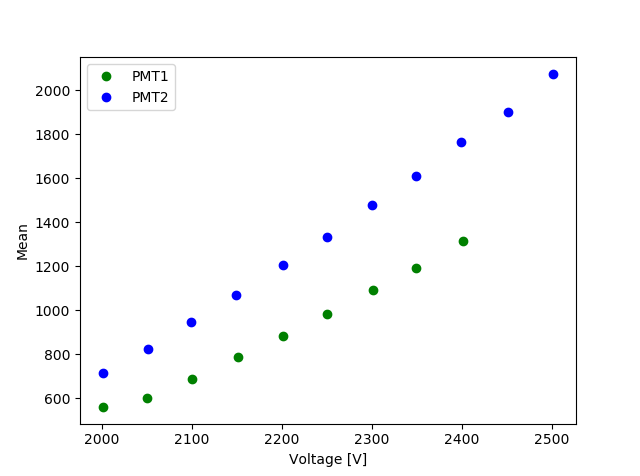
\includegraphics[scale=0.6]{mean.png}
\centering
\caption{Mean as a function of the voltage for both PMT.}
\label{fig:mean}
\end{figure}

Since for both PMTs we are in the linearity region, we can choose any desired voltage without restriction between 2000 V and 2500 V. This is the reason why we take into account the resolution of the PMTs. For computing the resolution we use the relation

\begin{equation}
    R = \frac{\sigma}{\Delta\mu},
\end{equation}

where $\sigma$ is the standard deviation and $\Delta\mu$ is the difference between the mean of the Gaussian of the second peak and the mean of the Gaussian of the background (as presented in Figures~\ref{fig:bck1} and~\ref{fig:bck2}). Figure \ref{fig:res} presents the resolution as a function of the high voltage for both PMTs.

\begin{figure}[H]
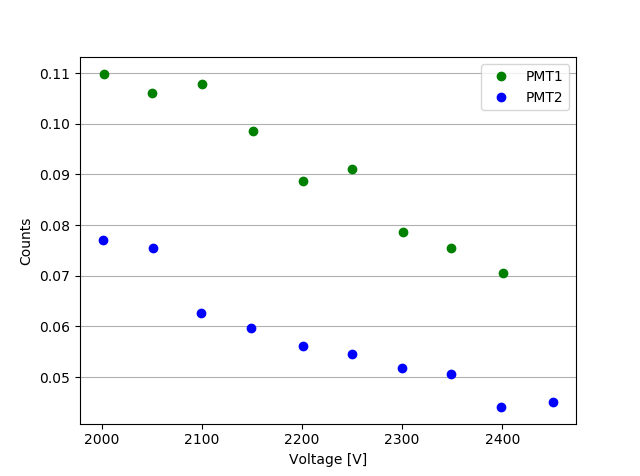
\includegraphics[scale=0.6]{Resolution.png}
\centering
\caption{Resolution as a function of the voltage for both PMT.}
\label{fig:res}
\end{figure}

By analysing this plot we can choose the best working voltage for each PMT. The tension is set to be 2200 V for the PMT1 and 2250 V for PMT2.\\

Figures \ref{fig:coin1} and \ref{fig:coin2} show the rate of the coincidences as a function of the high voltage for each PMT, while keeping the other fixed at 2350 V. At 2200 V in the PMT1 and 2250 V in PMT2 the rate blows up because the high voltage in the PMTs multiplies the number of electrons created (gain). Therefore it is found found that the optimal voltage is well outside the region of the plateau. In order to find a stable region around the set voltages it is necessary to change the discriminator parameters, the threshold and the width.

\begin{figure}[H]
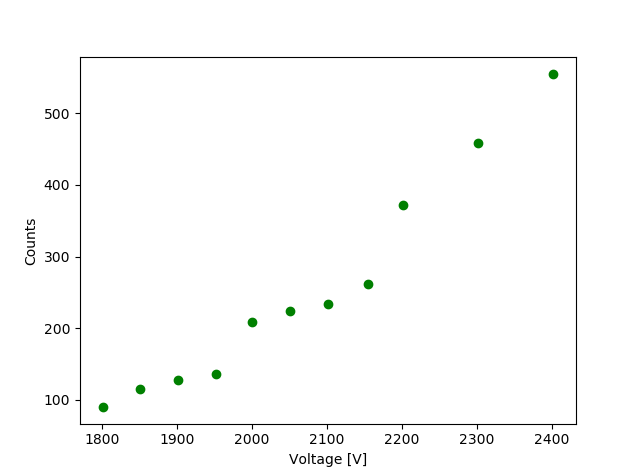
\includegraphics[scale=0.6]{CoincidencePMT1.png}
\centering
\caption{Coincidence as a function of voltage in PMT1 with PMT2 fixed at 2351 V.}
\label{fig:coin1}
\end{figure}

\begin{figure}[H]
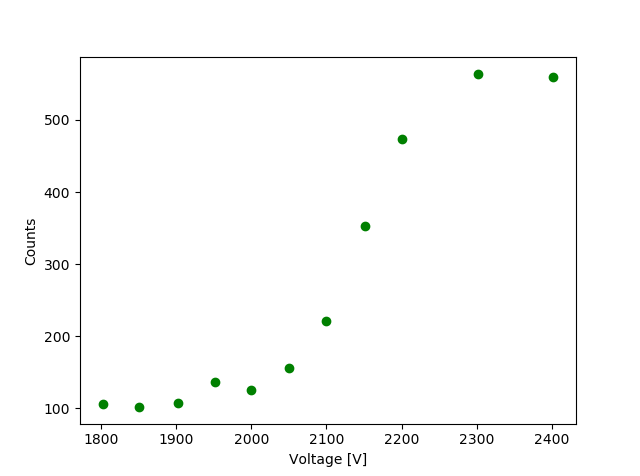
\includegraphics[scale=0.6]{CoincidencePMT2.png}
\centering
\caption{Coincidence as a function of voltage in PMT2 with PMT1 fixed at 2349 V.}
\label{fig:coin2}
\end{figure}

In order to set the voltage within the plateau the threshold of the discriminator has been changed to 150 mV.\\

By studying the coincidences as a function of the width of the discriminator we can conclude that when the width is too small no coincidences are observed. By increasing the width, we reach the plateau and for even higher values too many coincidences are counted and the rate of the coincidences quickly increase similarly for what happened with the coincidences as a function of the voltage. As a result, the width has been chosen to be 30 ns, in order to avoid accidental coincidences.\\

With the voltage already set, the last step is to find the channel-energy equivalence. Because of the electronics we have the results in ADC not in energy, therefore we need to convert it into energy. For doing that, first of all we have to assume a linear dependence between the ADC channel and the detector response. The second one regards the zero of the PMTs, called pedestal.\\

As shown in Figures~\ref{fig:bck1} and \ref{fig:bck2}, the background distribution (obtained from measurements without the source) presents a very narrow peak. It has been fitted with a Gaussian, which ADC value corresponds to energy's zero value.

\begin{figure}[H]
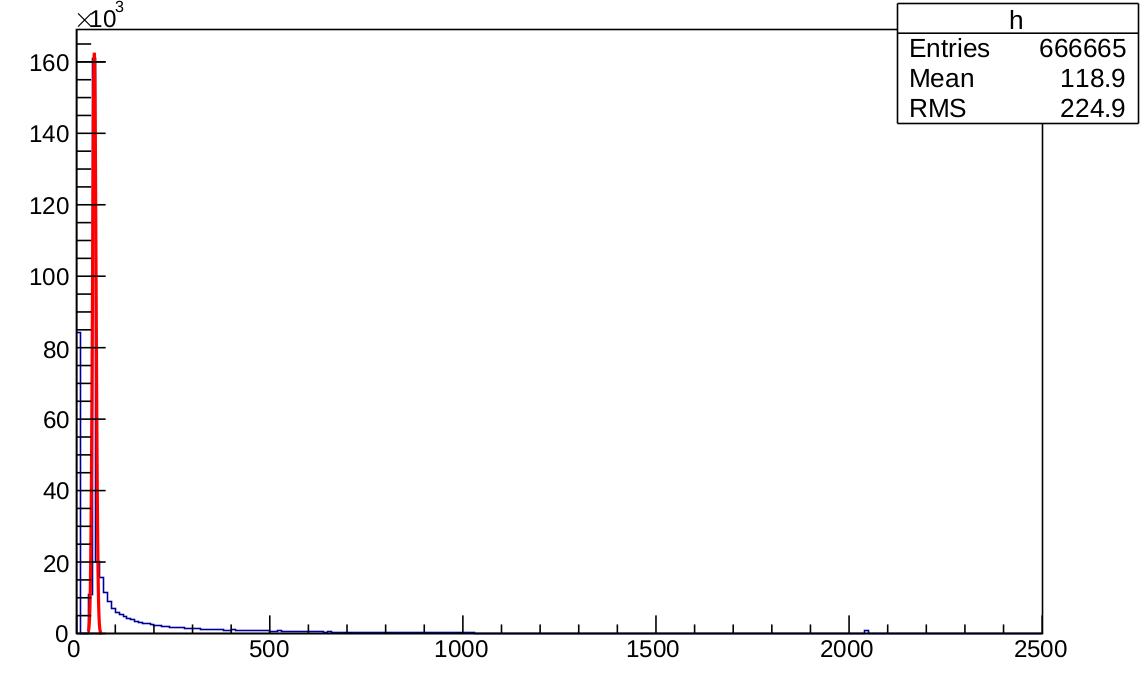
\includegraphics[scale=0.3]{background1.png}
\centering
\caption{Background signal distribution for PMT1 at 2201 V.}
\label{fig:bck1}
\end{figure}

\begin{figure}[H]
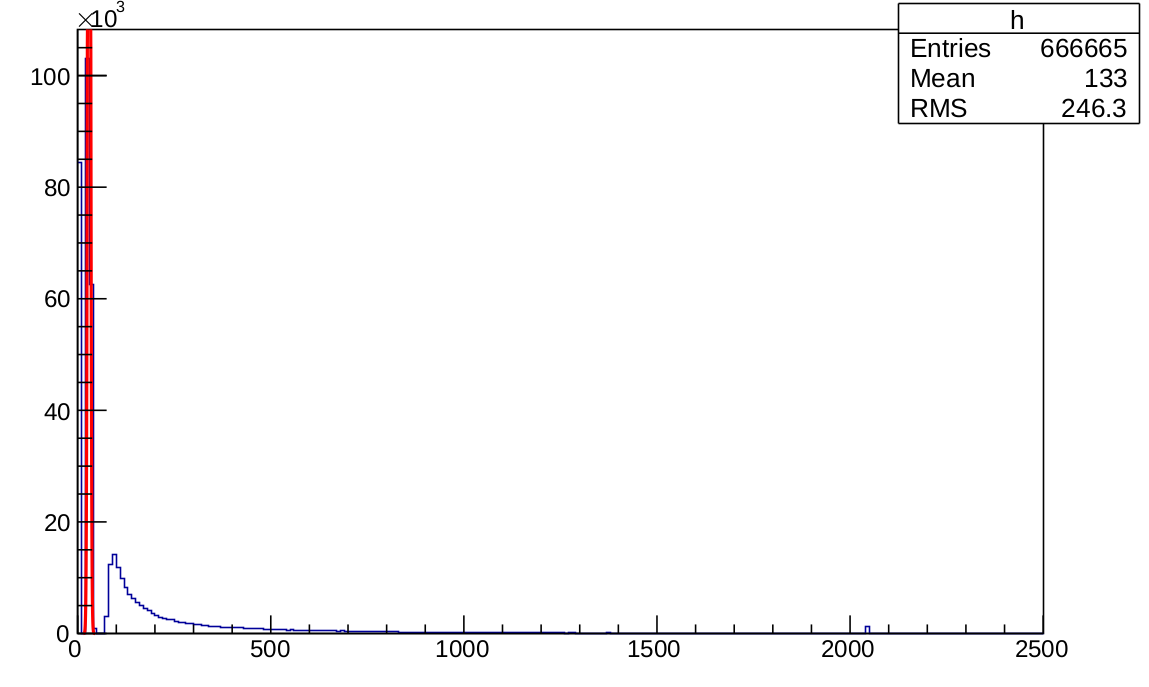
\includegraphics[scale=0.3]{background2.png}
\centering
\caption{Background signal distribution for PMT2 at 2250 V.}
\label{fig:bck2}
\end{figure}

For PMT1 the ADC for zero energy value is 45, while for PMT2 is 30.\\

In Figure~\ref{fig:spectrum}, as mentioned before, we discuss the spectrum of a $\prescript{207}{}{Bi}$ source. We know the energy of the peaks, so  we can establish a linear relation between this energy (1.06 \MeV) and the ADC channel for each photomultiplier. For doing that we fitted the measurement of the PMT1 at 2200 V and the PMT2 at 2250 V, as we can see in Figures \ref{fig:pmt1} and \ref{fig:pmt2}.

\begin{figure}[H]
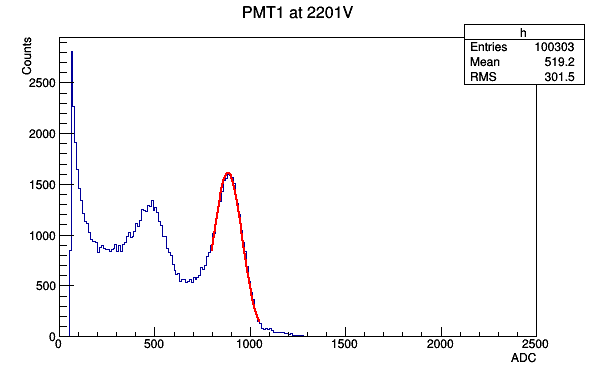
\includegraphics[scale=0.5]{PMT1_2201V.png}
\centering
\caption{Spectrum of the Bismuth source for the PMT1 at 2201 V with second peak fitted with a Gaussian.}
\label{fig:pmt1}
\end{figure}

\begin{figure}[H]
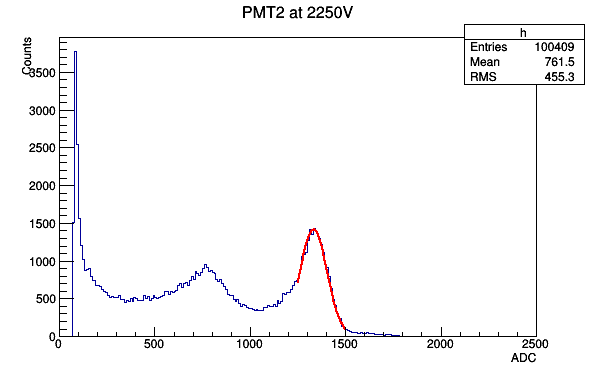
\includegraphics[scale=0.5]{PMT2_2250V.png}
\centering
\caption{Spectrum of the Bismuth source for the PMT2 at 2250 V with second peak fitted with a Gaussian.}
\label{fig:pmt2}
\end{figure}

The mean of the fitted peak for the PMT1 (Figure \ref{fig:pmt1}) is 885, for the PMT2 (Figure \ref{fig:pmt2}) is 1334. Therefore the linear relation for each one is given respectively by

\begin{equation}
    E_1 (\MeV) = 0.0013 \cdot {\rm ADC} - 0.058,
\end{equation}

\begin{equation}
    E_2 (\MeV) = 0.00081 \cdot {\rm ADC} - 0.024.
\end{equation}

\newpage

\section{The foil}

The foil used in this experiment is made of iron or aluminium (38 x 100 x 0.01 mm). Iron is a ferromagnetic material. It exhibits a strong magnetism in the same direction of the field, when a magnetic field is applied to it. Due to this characteristic we can study the coincidence as a function of its polarisation. Aluminium cannot be polarised, therefore it is used to prove that the experiment is unbiased.\\

The foil is placed between the radioactive source and the PMTs. The support for the foil is a metallic frame with two coils (Figure \ref{fig:cible}), which will allow the polarisation. The whole structure is fixed inside the enclosure. In order to measure the longitudinal polarisation of $\beta$ particles, target electrons should be polarised in the direction of incident electrons. Therefore, the foil is tilted with an angle of 30 degrees, allowing a longitudinal component of the polarisation, as illustrated in Figure~\ref{fig:30}.

\begin{figure}[H]
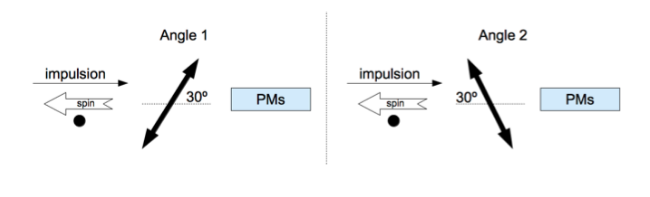
\includegraphics[scale=0.5]{Foil30.png}
\centering
\caption{Schematic of the two possible orientations of the foil}
\label{fig:30}
\end{figure}

In order to estimate the systematic errors due to possible asymmetries in the setup (in particular the effect of the magnetic field and the differences between the two PMTs), the foil will be placed in two different directions as shown in Figure~\ref{fig:cible}. \\

Moreover, we reverse the magnetic field every 5 minutes, since we reverse the direction of the current in the coils. In this way, the polarisation changes, which helps us to reach the goal of the experiment. That goal is to measure the number of electrons detected with polarisation up and with polarisation down, and check if it exists any asymmetry between them.

\subsection{Polarisation of the foil}\label{polfoil}

The aim of this section is to estimate the polarisation of the foil using its hysteresis cycle.\\

To polarise the foil we use an internal coil (red coils in Figure \ref{fig:cible}). It is connected to a signal generator, which provides a 2.7 kHz alternate signal. This signal induces a magnetic field in an external coil, placed around the foil.\\

The induced current passes through a RC circuit (Figure \ref{fig:int}). In this circuit the frequency is higher than its characteristic time, $\omega >>1/RC$, since $R = 10^4 \pm 5\%$ $\Omega$ and $  C = 10^{-6} \pm 20\%$ F, thus the circuit works as an integrator. 

\begin{figure}[H]
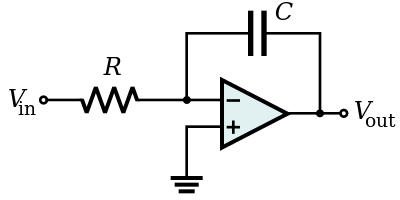
\includegraphics[scale=0.3]{integrator.png}
\centering
\caption{Diagram of the integrator.}
\label{fig:int}
\end{figure}

To simplify the calculations, we assume that the circuit is an ideal one, which means that the impedance is infinite. Therefore, the current in the capacitor is 

\begin{equation}
    I_C = C \frac{dV_C}{dt}.
\end{equation}

Since $I_{\rm out}=I_{\rm in}$, $V_C = V_{\rm out}$ and knowing Ohm law

\begin{equation}
    \Delta V_{\rm out}= \frac{1}{R C} \int V_{\rm in} dt
\end{equation}

, and by also using the Faraday-Neumann-Lenz law, we finally obtain
\begin{equation}
    \Delta V_{out}= \frac{1}{R C} \Delta \phi, 
\end{equation}

where $\phi$ is the flux crossing the coil, $\phi = B \cdot N \cdot S$, $B$ is the magnetic field, N is the number of turns in the coil and S is the surface.\\

Therefore the magnetic field is given by
\begin{equation}
    B = \frac{C \ R \ \Delta V_{\rm out}}{N \ S}.
\end{equation}

The coil has 1000 spires and a surface of $(4 \pm 0.1)\cdot 10^{-7}{\rm m}^2$. \\

From the hysteresis curve on the oscilloscope, illustrated in Figure~\ref{fig:curve}, we can extract the value of the tension, $\Delta V_{\rm out} = \frac{0.06}{2} = 3 \cdot 10^{-2}\  {\rm V}$.

\begin{figure}[H]
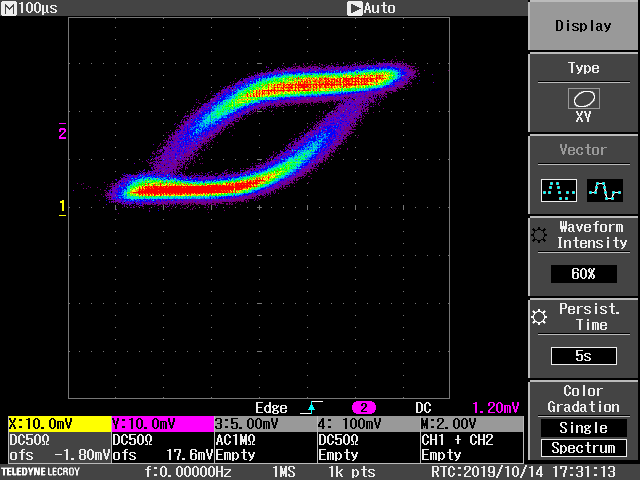
\includegraphics[scale=0.3]{SCRN0004.PNG}
\centering
\caption{Hysteresis curve of the iron foil.}
\label{fig:curve}
\end{figure}

Thus, the saturation field is

\begin{equation*}
    \mathbf{B = (0.75 \pm 0.3)T},
\end{equation*}

where the error has been computed by using the propagation of uncertainty formula.\\

The magnetisation of the foil and the field are related by the following relation: $B = \mu_0 (H+M)$. It can be approximated as $B \approx \mu_0 M$ , because of ferromagnetic properties of the iron.\\

The polarised electron fraction is related with the magnetisation as

\begin{equation}
    f = \frac{M}{\mu_B \rho} = \frac{B}{\mu_B \mu_0 \rho},
\end{equation}

where the Bohr magneton is $\mu_B = 9.27 \cdot 10^{-24} {\rm JT}^{-1}$, the vacuum permeability is $\mu_0 = 4 \pi \cdot 10^{-7} {\rm TmA}^{-1}$, and $\rho$ is the polarised electrons density. Since only the external electrons contribute to the magnetisation (2 electron per atom), we can compute easily the number of iron atoms as $\rho = (1.69 \pm 0.02) \cdot 10^{-30} e^-{\rm m}^{-3}$.\\

Again, using the propagation of uncertainty formula, we conclude

\begin{equation*}
    \mathbf{f = (3.8 \pm 1.14)\%}
\end{equation*}

\chapter{Data analysis}

\section{Analysis}

As we explained in the previous Section \ref{asym}, we want to verify the parity violation of the weak interaction, which has a vector-axial nature. We need to measure the count rate of the asymmetry with the Equations \ref{27} and \ref{30}. We can modify the last equation in such a way that the variable will be the number of events detected
\begin{equation}\label{epsi}
   \epsilon = \frac{N_{\rm up}-N_{\rm down}}{N_{\rm up}+N_{\rm down}} .
\end{equation}

The data have been divided in five independent data sets. The first three of them have been taken with the orientation of the foil as shown in the left part of the Figure \ref{fig:30}, the remaining data set, with the opposite orientation.\\

First of all, we need to determine the energy range accessible in the experiment. Since the PMTs are placed at an angle of $35\pm 11 ^o$, only the electrons with a range of energies from 0.2 \MeV~up tp 2.3 \MeV, are able to exist.\\

In order to improve the quality of the analysis, further requirements have been implemented. Namely, the absolute value of the energy difference for each PMT has to be less than 0.4 \MeV.

\begin{figure}[H]
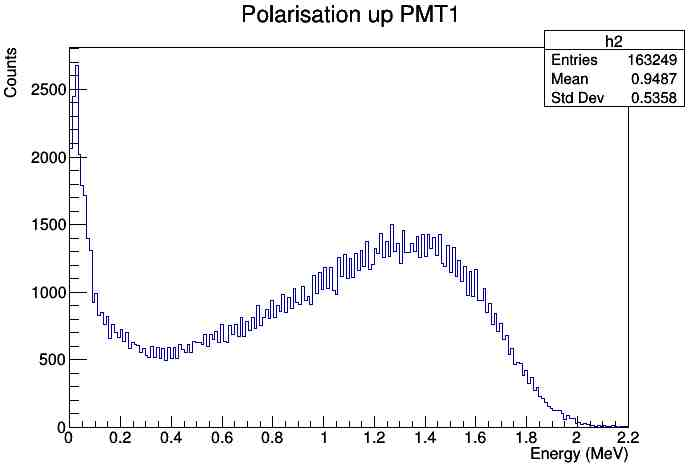
\includegraphics[scale=0.3]{upPMT1.jpg}
\centering
\caption{Spectrum energy for polarisation up for the PMT1.}
\label{fig:up}
\end{figure}

In the Figure \ref{fig:up} it is shown the number of events as a function of the energy for the PMT1 for the polarisation up of the foil. We can see that the first peak is the most important contribution to the statistics. Otherwise we are interested in the second one. Therefore, we need to apply a cut for the region with larger energy than 0.4 MeV.

\begin{figure}[H]
\begin{subfigure}{.5\textwidth}
  \centering
  % include first image
  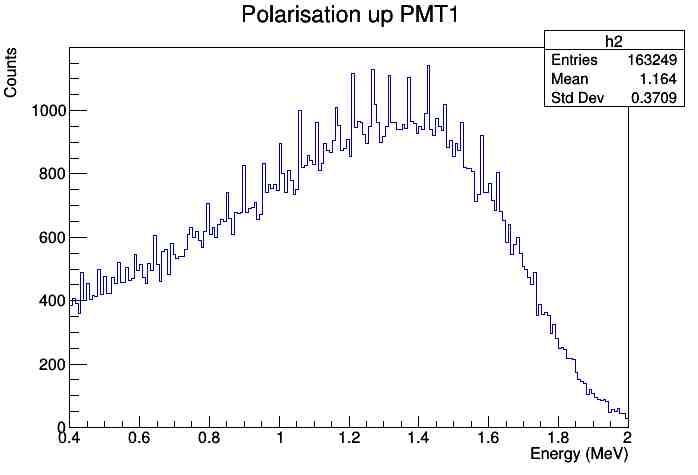
\includegraphics[width=.8\linewidth]{upPMT1cut.jpg}  
  \caption{Polarisation up for PMT1 in the interval [0.4-2.0].}
  \label{fig:upcut}
\end{subfigure}
\begin{subfigure}{.5\textwidth}
  \centering
  % include second image
  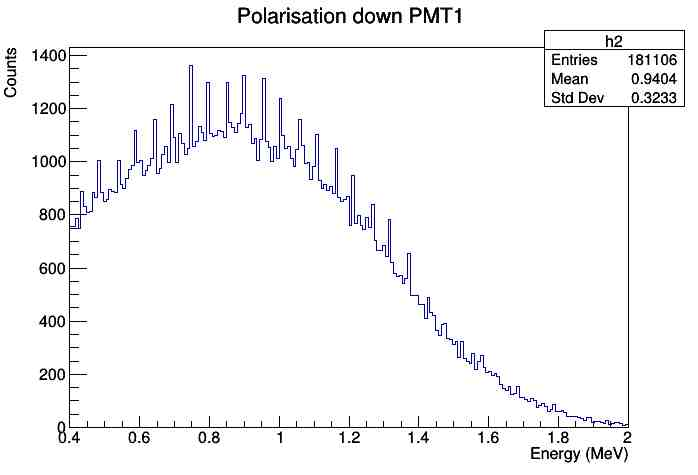
\includegraphics[width=.8\linewidth]{downPMT1cut.jpg}  
  \caption{Polarisation down for PMT1 in the interval [0.4-2.0].}
  \label{fig:downcut}
\end{subfigure}
\caption{Polarisation for PMT1 and PMT2 with a cut between 0.4 \MeV~and 2.0 \MeV.}
\label{fig:fig}
\end{figure}

Figures \ref{fig:upcut} and \ref{fig:downcut} show the region of interest for the two polarisation of the foil detected by PMT1. In these two figures, we can also observe that the maximum value is higher for polarisation up. However, the number of electrons detected for down polarisation is higher than the number detected for up polarisation.\\

In Figures \ref{fig:Poldown} and Figure \ref{fig:Polup}, it is shown 2D plots of the coincidences as a function of the energy in both PMTs. We can see that there is a difference in the number of detection depending on the polarisation applied. It is part of a systematic error. The magnetic field that deviates the electrons and their trajectories are favoured by one of the PMT. This is not a problem, since this preference changes with the polarisation, therefore, we can consider it null in average.

\begin{figure}[H]
\begin{subfigure}{.5\textwidth}
  \centering
  % include first image
  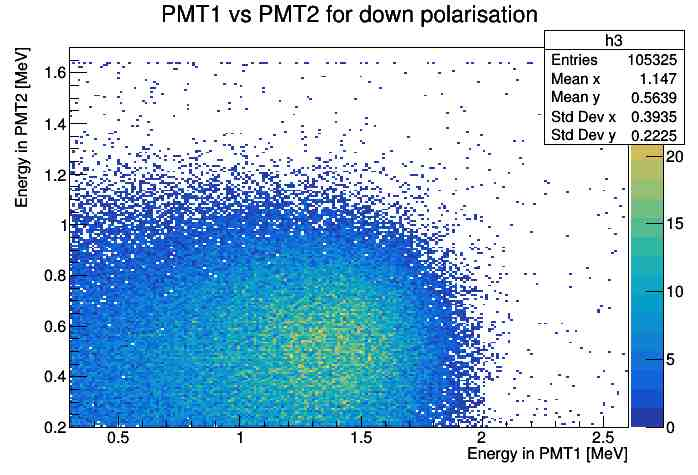
\includegraphics[width=.8\linewidth]{downPolX.jpg}  
  \caption{Coincidence distribution for down polarisation.}
  \label{fig:Poldown}
\end{subfigure}
\begin{subfigure}{.5\textwidth}
  \centering
  % include second image
  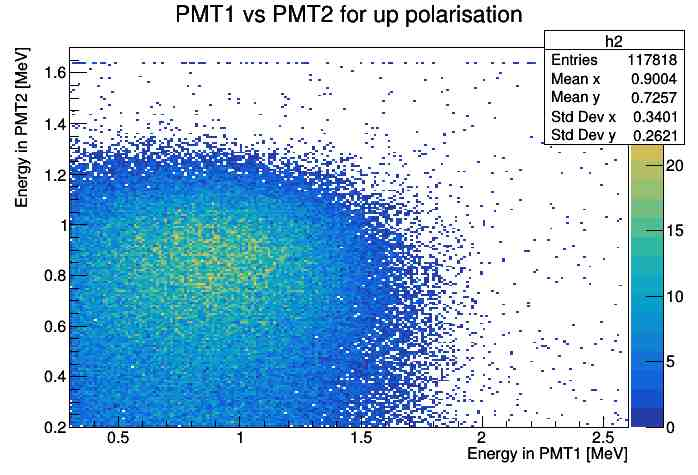
\includegraphics[width=.8\linewidth]{UPPolX.jpg}  
  \caption{Coincidence distribution for up polarisation.}
  \label{fig:Polup}
\end{subfigure}
\caption{2D distribution of the coincidences as a function of the energy of both PMTs for the Iron foil.}
\label{fig:fig}
\end{figure}

In Figures \ref{fig:unup} and \ref{fig:undown} we can see the distributions of the coincidence as a function of the energy in both PMTs of the Aluminium foil.

\begin{figure}[H]
\begin{subfigure}{.5\textwidth}
  \centering
  % include first image
  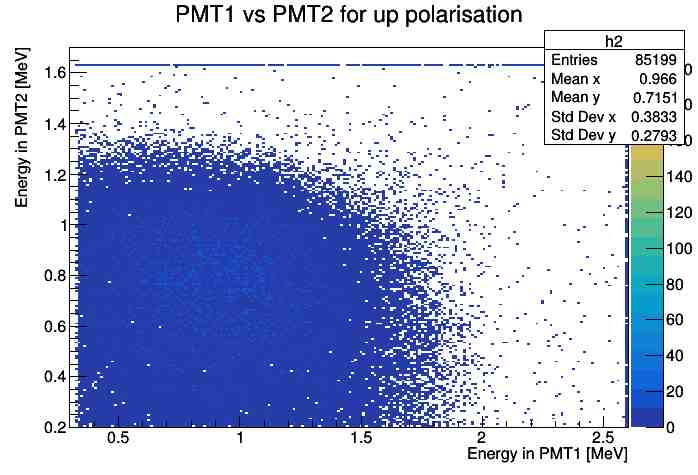
\includegraphics[width=.8\linewidth]{unpolup.jpg}  
  \caption{Coincidence distribution for up polarisation.}
  \label{fig:unup}
\end{subfigure}
\begin{subfigure}{.5\textwidth}
  \centering
  % include second image
  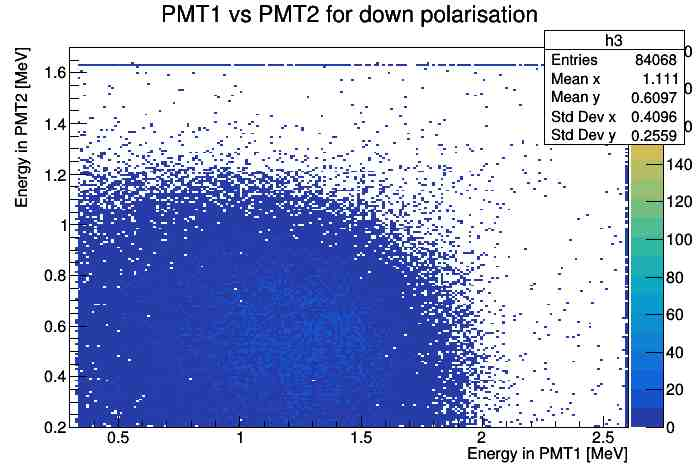
\includegraphics[width=.8\linewidth]{unPoldown.jpg}  
  \caption{Coincidence distribution for down polarisation.}
  \label{fig:undown}
\end{subfigure}
\caption{2D distribution of the coincidences as a function of the energy of both PMTs of the Aluminium foil.}
\label{fig:unpol}
\end{figure}

\section{Results}

\subsection{Asymmetry}

With the Formula~\ref{epsi} and the measurements done, we can compute the asymmetry. We made a cut in the data, in order to only take into account the values for the coincidence with energies above 0.4 \MeV. Figure \ref{fig:asymfit} show the value of the asymmetry for the different data sets.

\begin{figure}[H]
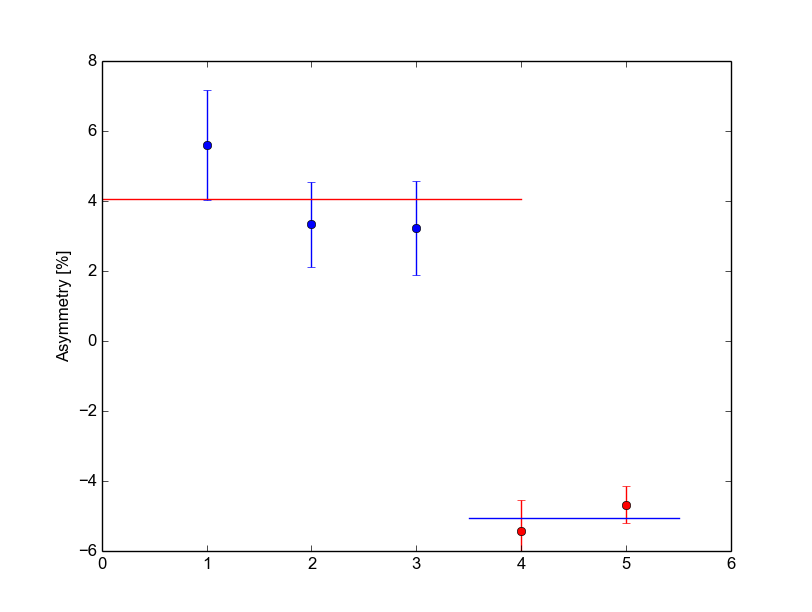
\includegraphics[scale=0.3]{epsilon.png}
\centering
\caption{Value of the asymmetry for different data sets, fitted with a constant function.}
\label{fig:asymfit}
\end{figure}

The asymmetry for the different data sets have been extrapolated with a constant function. The statistical uncertainty has been taken from the fit and the systematic uncertainty has been estimated as the difference between the two values of the fit. \\

The final result is 

\begin{equation*}
    \mathbf{\epsilon = (4.56 \pm 0.92 (stat) \pm 0.5 (sys))\%}.
\end{equation*}

We can see that the asymmetry is different from zero, therefore, there is a parity violation in the weak interactions.\\

Using the same formula we can compute the asymmetry for the Aluminium foil as

\begin{equation*}
    \mathbf{\epsilon = (0.6 \pm 0.43 (stat))\%}.
\end{equation*}

In this case, we cannot estimate the systematic error since we only used one orientation of the foil. For the statistical uncertainty, we use the same idea as before. It comes from the fit (average between two points). We can conclude with this result that is compatible with zero. Therefore, there is no asymmetry and it confirms the parity violation.

\subsection{Polarisation} 

Once that the parity violation has been shown, it is possible to compute the polarisation of the decay electrons.\\

Using the Equation \ref{30} discussed in section \ref{asym}, where $P_{\rm s}$ is the longitudinal polarisation of the electrons emitted by the source and $P_{\rm t}$, the longitudinal polarisation of the electrons in the target. Since the foil is tilted $30^o$, $P_{\rm t} = f\cdot \cos(30^o)$. As a consequence we obtain the following relation

\begin{equation}\label{Ps}
    P_{\rm s} = \frac{\epsilon}{f \cdot \cos(30^o) \cdot A(\theta, \beta)}.
\end{equation}

Equation \ref{Ps} is true for a single energy, scattering angle, and angle between the trajectory of the electron and the foil. The problem of averaging the expression is, in general, very complicated. It is simplified if the accept energy range is reasonably narrow. In particular, we consider $A(\theta, \beta)=1$ because the diffusion angle is $\theta = \pi/2$ and the electron do not have a relativistic speed.\\

The polarisation of the target,$f=(3.8 \pm 1.14)\%$, computed in section \ref{polfoil}, give sus the final result for the polarisation as

\begin{equation*}
    \mathbf{ P_{\rm s} = (137 \pm 33 (foil) \pm 2 (sys))\%},
\end{equation*}

where the error called foil is due to the propagation errors where we also take into account the error on the asymmetry, and the systematic is computed for the different values of the asymmetry observed.


\chapter{Conclusion}

The values that we have measured during this experiment demonstrate that parity is violated in weak interactions, in concordance with the theory. The experiment allows us to compute the number of electrons polarised in the source, thus the number of electrons polarised in the foil.

The summary of the values obtained in this experiment are presented the Table~\ref{tab:summary}.

\begin{table}[H]
    \centering
    \begin{tabular}{|c |c|}
    \hline
         $\mathbf{B [T]}$ & $\mathbf{0.75 \pm 0.3}$ \\
         \hline
         $\mathbf{f [\%]}$ & $\mathbf{3.8 \pm 1.14}$\\
         \hline
         $\mathbf{\epsilon [\%]}$ & $\mathbf{4.56 \pm 0.92 (stat) \pm 0.5 (sys)}$\\
         \hline
        $\mathbf{P_{\rm s} [\%]}$ & $\mathbf{137 \pm 33(foil) \pm 2(sys)}$\\ 
        \hline
    \end{tabular}
    \label{tab:summaryl}
    \caption{Summary of values obtained}
\end{table}

The main source of error arises from the polarisation of the foil. Since the large uncertainty associated to the measurement of the magnetic field (Subsection \ref{polfoil}). We had several problems for measuring the hysteresis curve of the foil and we think that the system should be improve. A flux-meter can be used to measure the magnetic flux with and without the foil, the difference between these two measurement will give the foil contribution.\\

Despite our large uncertainty and a bit higher numbers for the polarisation, they are compatible with the theoretical ones.

\pagebreak


% Adding a bibliography if citations are used in the report
\bibliographystyle{plain}
\bibliography{BiBTeXexempel.bib}
\begin{thebibliography}{}
\bibitem{}
http://dpnc.unige.ch/~bravar/PPA2/PPA2-L10.pdf

\bibitem{}
http://dpnc.unige.ch/~bravar/PPA2/PPA2-L9.pdf
\bibitem{}
http://dpnc.unige.ch/~bravar/PPA2/PPA2-L8.pdf
\bibitem{}
http://dpnc.unige.ch/~bravar/PPA2/PPA2-L7.pdf
\bibitem{}
 Modern particle physics - Thomson, Mark 
 \bibitem{}
 A Modern Introduction to Quantum. Field Theory. Michele Maggiore
 \bibitem{}
 http://archive.is/NhDVF
 \bibitem{}
 http://archive.is/NhDVF\#selection-777.0-777.36
 \bibitem{}
 https://ocw.mit.edu/courses/physics/8-01sc-classical-mechanics-fall-2016/readings/MIT8\_01F16\_chapter15.pdf
 \bibitem{}
 http://www.radioactivity.eu.com/site/pages/Strontium\_90.htm
 \bibitem{}
 https://www.sciencedirect.com/topics/physics-and-astronomy/photomultiplier-tubes
 \bibitem{}
 https://www.bipm.org/cc/CIPM/Allowed/96/CIPM09\_Materials\_WG\_Report\_Part\_2.pdf
 \bibitem{}
  Determination of Electron and Positron Helicity with Moller and Bhabha Scat- tering,J.D. Ullman et al
  \bibitem{violation}
    Robert Novick.Thirty Years Since Parity Nonconservation, A Symposium for T.D. Lee. Bri-khäuser, 1988.
    \bibitem{paritos}
    H. Frauenfelder, A. O. Hanson, N. Levine, A. Rossi, and G. DePasquali.Phys. Rev. 107 643
    \bibitem{parity}
    T. D. Lee and C. N. Yang.Phys. Rev. 104 254.
 \end{thebibliography}
% Adds reference to the Bibliography in the ToC
\addcontentsline{toc}{chapter}{\bibname}


\end{document}

